
%============================================================
\subsection{\texttt{dogbone}}
\label{subsec:geometry_dogbone}
%============================================================

\noindent
\textbf{Geometry ID:} \texttt{GLOB-GEO0005}
\qquad
\textbf{Version:} \texttt{1.0.0}

\begin{figure}[htbp]
    \centering
    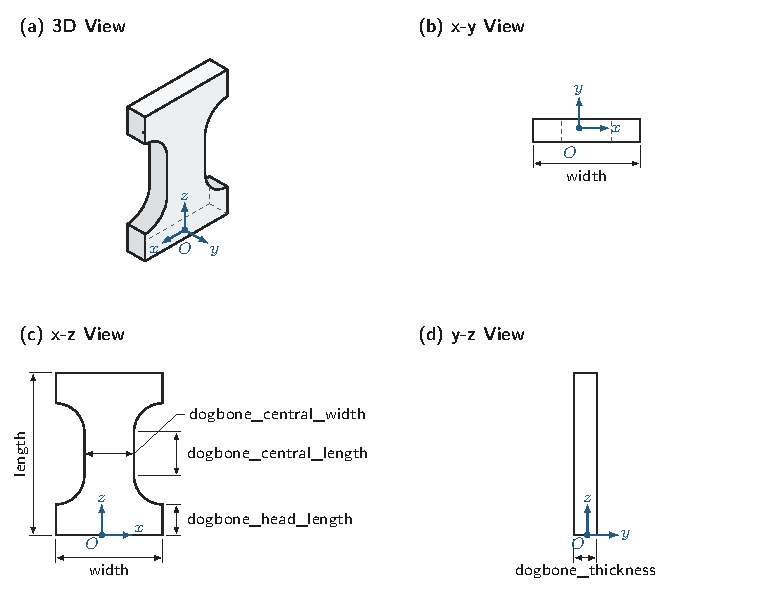
\includegraphics[width=0.65\linewidth]
    {./figs/geometries/dogbone.pdf}
    \caption{Standardized parametrization and local
    coordinate system of the dogbone geometry.}
    \label{fig:dogbone}
\end{figure}

The \texttt{dogbone} geometry represents a specimen
consisting of two identical enlarged heads connected
to a reduced central region through two identical
transition regions.

As illustrated in Fig.~\ref{fig:dogbone}, the
local coordinate system is defined by the
right-handed Cartesian axes $x$, $y$, and $z$,
with the origin located at the reference point
indicated in the figure.

The $z$ axis represents the longitudinal direction,
the $x$ axis the specimen width direction,
and the $y$ axis the thickness direction.

\paragraph{Independent parameters.}

The geometry is defined by six required dimensional
parameters, expressed in millimeters, and one
optional categorical parameter:

\begin{itemize}
    \item \texttt{length}: overall specimen length
    along the local $z$ axis;

    \item \texttt{width}: maximum specimen width,
    measured across the enlarged heads along
    the local $x$ axis;

    \item \texttt{dogbone\_central\_length}:
    longitudinal length of the reduced central
    region;

    \item \texttt{dogbone\_central\_width}:
    width of the reduced central region;

    \item \texttt{dogbone\_head\_length}:
    longitudinal length of each enlarged head;

    \item \texttt{dogbone\_thickness}:
    specimen thickness along the local $y$ axis;

    \item \texttt{transition\_type}:
    optional categorical parameter defining
    the shape of the transition regions.
    Permitted values are
    \texttt{linear\_transition} and
    \texttt{curved\_transition}.
    The default is \texttt{curved\_transition}.
\end{itemize}

The transition type specifies whether the lateral
boundaries connecting the enlarged heads to the
reduced central region are linear or curved.
For curved transitions, the precise curvature
is not prescribed by the current parametrization.

\paragraph{Derived parameters.}

The longitudinal length of each transition region
is determined by

\begin{equation}
\begin{aligned}
\texttt{dogbone\_transition\_length}
= \frac{1}{2}\bigl(
&\texttt{length}
-2\,\texttt{dogbone\_head\_length}\\
&-\texttt{dogbone\_central\_length}
\bigr).
\end{aligned}
\end{equation}

The lateral width reduction on each side of the
specimen is given by

\begin{equation}
\begin{aligned}
\texttt{dogbone\_transition\_width}
=\frac{1}{2}\bigl(
&\texttt{width}\\
&-\texttt{dogbone\_central\_width}
\bigr).
\end{aligned}
\end{equation}

These quantities are derived from the independent
parameters and are not specified separately.

\paragraph{Geometric constraints.}

All required dimensional parameters must be
strictly positive. In addition, the geometry
must satisfy

\begin{align}
\texttt{length}
&>
2\,\texttt{dogbone\_head\_length}
+\texttt{dogbone\_central\_length},
\\
\texttt{width}
&>
\texttt{dogbone\_central\_width}.
\end{align}

These conditions ensure strictly positive
transition lengths and lateral width reductions.
